% Matrix product operator drawn as a tensor network (Session 5).
% Own drawing. Compile with: pdflatex mpo_chain.tex ; result moves to ../mpo_chain.pdf
\documentclass[11pt,tikz,border=3pt]{standalone}
\usepackage{amsmath,amssymb}
\usepackage{xcolor}
\definecolor{coursedark}{HTML}{1B2A4A}
\definecolor{courseaccent}{HTML}{7A2E8C}

\begin{document}
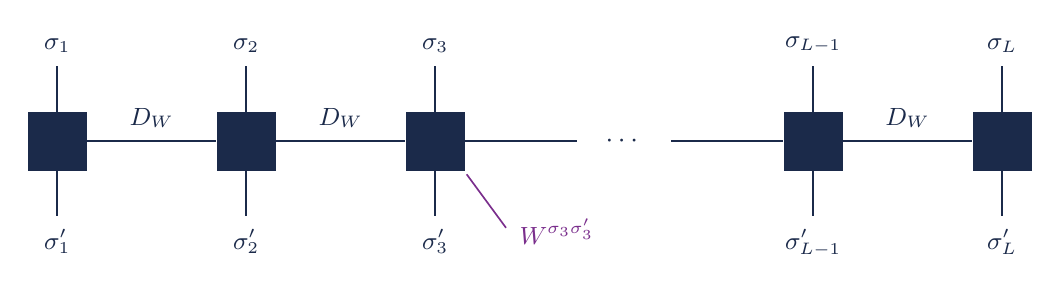
\begin{tikzpicture}[
    optensor/.style={rectangle, fill=coursedark, minimum size=7.5mm, inner sep=0pt},
    wire/.style={draw=coursedark, line width=0.9pt},
    lbl/.style={font=\small, text=coursedark},
  ]

  \def\leg{0.95}

  % ---- site tensors, one row index up and one column index down
  \foreach \i/\x/\up/\dn in {%
      1/0/{\sigma_1}/{\sigma_1'},
      2/2.4/{\sigma_2}/{\sigma_2'},
      3/4.8/{\sigma_3}/{\sigma_3'},
      4/9.6/{\sigma_{L-1}}/{\sigma_{L-1}'},
      5/12.0/{\sigma_L}/{\sigma_L'}} {
    \node[optensor] (w\i) at (\x,0) {};
    \draw[wire] (\x,0.375) -- (\x,\leg);
    \draw[wire] (\x,-0.375) -- (\x,-\leg);
    \node[lbl, anchor=south] at (\x,\leg+0.05) {$\up$};
    \node[lbl, anchor=north] at (\x,-\leg-0.05) {$\dn$};
  }

  % ---- internal bond legs
  \draw[wire] (w1) -- (w2) node[lbl, midway, above=1pt] {$D_W$};
  \draw[wire] (w2) -- (w3) node[lbl, midway, above=1pt] {$D_W$};
  \draw[wire] (w4) -- (w5) node[lbl, midway, above=1pt] {$D_W$};

  % ---- the part of the chain we are not drawing
  \draw[wire] (w3) -- (6.6,0);
  \node[text=coursedark] at (7.2,0) {$\cdots$};
  \draw[wire] (7.8,0) -- (w4);

  % ---- what a bulk tensor is
  \node[lbl, anchor=west, text=courseaccent] at (5.75,-1.15) {$W^{\sigma_3\sigma_3'}$};
  \draw[courseaccent, line width=0.6pt] (5.7,-1.1) -- (5.2,-0.42);

\end{tikzpicture}
\end{document}
